% Neural SINDy presentation slides
% Built on the Elegant Slides template by Lars Spreng (CC BY 4.0)

\documentclass[
11pt,notheorems,hyperref={pdfauthor=Aniruddha Pandey}
]{beamer}

\input{loadslides.tex}

\graphicspath{{../}}

\title[Neural SINDy]{Neural SINDy: Sparse System Identification\\with Grokked MLP Libraries}

\author[Aniruddha Pandey]{Aniruddha Pandey}

\institute{
    Department of Computer Science\\
    Stevens Institute of Technology
}
\date{\today}

\begin{document}

% Title page
{
\setbeamertemplate{footline}{}
\begin{frame}
  \titlepage
\end{frame}
}
\addtocounter{framenumber}{-1}

\begin{frame}{Outline}{}
    \footnotesize
    \begin{columns}[T,onlytextwidth]
        \column{0.46\textwidth}
            \textbf{Part I: Motivation and Background}\par\smallskip
            \tableofcontents[part=1,hideallsubsections]
            \medskip
            \textbf{Part II: Method}\par\smallskip
            \tableofcontents[part=2,hideallsubsections]
        \hspace{0.04\textwidth}
        \column{0.46\textwidth}
            \textbf{Part III: Experiments and Results}\par\smallskip
            \tableofcontents[part=3,hideallsubsections]
            \medskip
            \textbf{Part IV: Wrap-up}\par\smallskip
            \tableofcontents[part=4,hideallsubsections]
    \end{columns}
\end{frame}

\makepart{Motivation and Background}

\section{Motivation}

\begin{frame}{The Problem}
\begin{itemize}
    \item \emphasize{Goal:} discover the governing equations of a physical system from noisy measurements.
    \item \textbf{Running toy example:} a damped spring,
    \begin{equation*}
        \ddot{x} = -k x - c \dot{x}.
    \end{equation*}
    \item You measure position $x(t)$ and velocity $v(t)$ but \alert{do not know} the equation.
    \item Can the data tell you it is a spring?
\end{itemize}
\end{frame}

\section{Background: SINDy}

\begin{frame}{What SINDy Does}
Frame equation discovery as sparse regression:
\begin{equation*}
    \dot{\mathbf{X}} = \boldsymbol{\Theta}(\mathbf{X})\,\boldsymbol{\Xi}
\end{equation*}
\begin{itemize}
    \item $\boldsymbol{\Theta}$ -- a \emphasize{library} of candidate functions
    \item $\boldsymbol{\Xi}$ -- a \emphasize{sparse} coefficient vector
\end{itemize}
\textbf{Toy library:} $[\,1,\; x,\; v,\; x^2,\; xv,\; \sin(x)\,]$\\[0.3cm]
\textbf{Hoped-for outcome:}
$\boldsymbol{\Xi} = [0,\,-2.0,\,-0.3,\,0,\,0,\,0] \;\Rightarrow\; \dot{v} = -2x - 0.3v$
\end{frame}

\begin{frame}{SINDy's Three Pain Points}
\begin{enumerate}
    \item \alert{Library must be specified up front.} If $\sin$ is missing but the truth needs $\sin$, SINDy returns a confidently wrong fit.
    \item \alert{Combinatorial explosion.} Higher-order or composed functions blow up library size.
    \item \alert{Noise sensitivity.} Rigid analytical primitives do not absorb sensor noise gracefully.
\end{enumerate}
\vspace{0.4cm}
This work attacks all three by \emphasize{replacing the library with neural networks}.
\end{frame}

\section{Core Idea}

\begin{frame}{The Core Idea}
Replace each library entry with a small MLP trained to ``grok'' a math operation:
\begin{equation*}
\sin(x) \to \mathrm{sin\_mlp}(x), \quad x+y \to \mathrm{add\_mlp}(x,y), \;\dots
\end{equation*}
\textbf{Why this could help:}
\begin{itemize}
    \item MLPs are \emphasize{differentiable end-to-end} -- enables gradient-based selection.
    \item Smooth approximations may \emphasize{absorb noise better}.
    \item Symbolic interpretability recovered later via \example{PySR distillation}.
\end{itemize}
\end{frame}

\subsection{Grokking}

\begin{frame}{Primer: Grokking}
\begin{itemize}
    \item \emphasize{Grokking}: validation loss drops sharply long after training loss has plateaued.
    \item Tiny MLPs (128 hidden, Tanh) trained with AdamW + heavy weight decay until val MSE $\approx 10^{-7}$.
    \item Used \alert{descriptively} -- not claiming the same mechanism as the original modular-arithmetic paper.
\end{itemize}
\begin{figure}
    \centering
    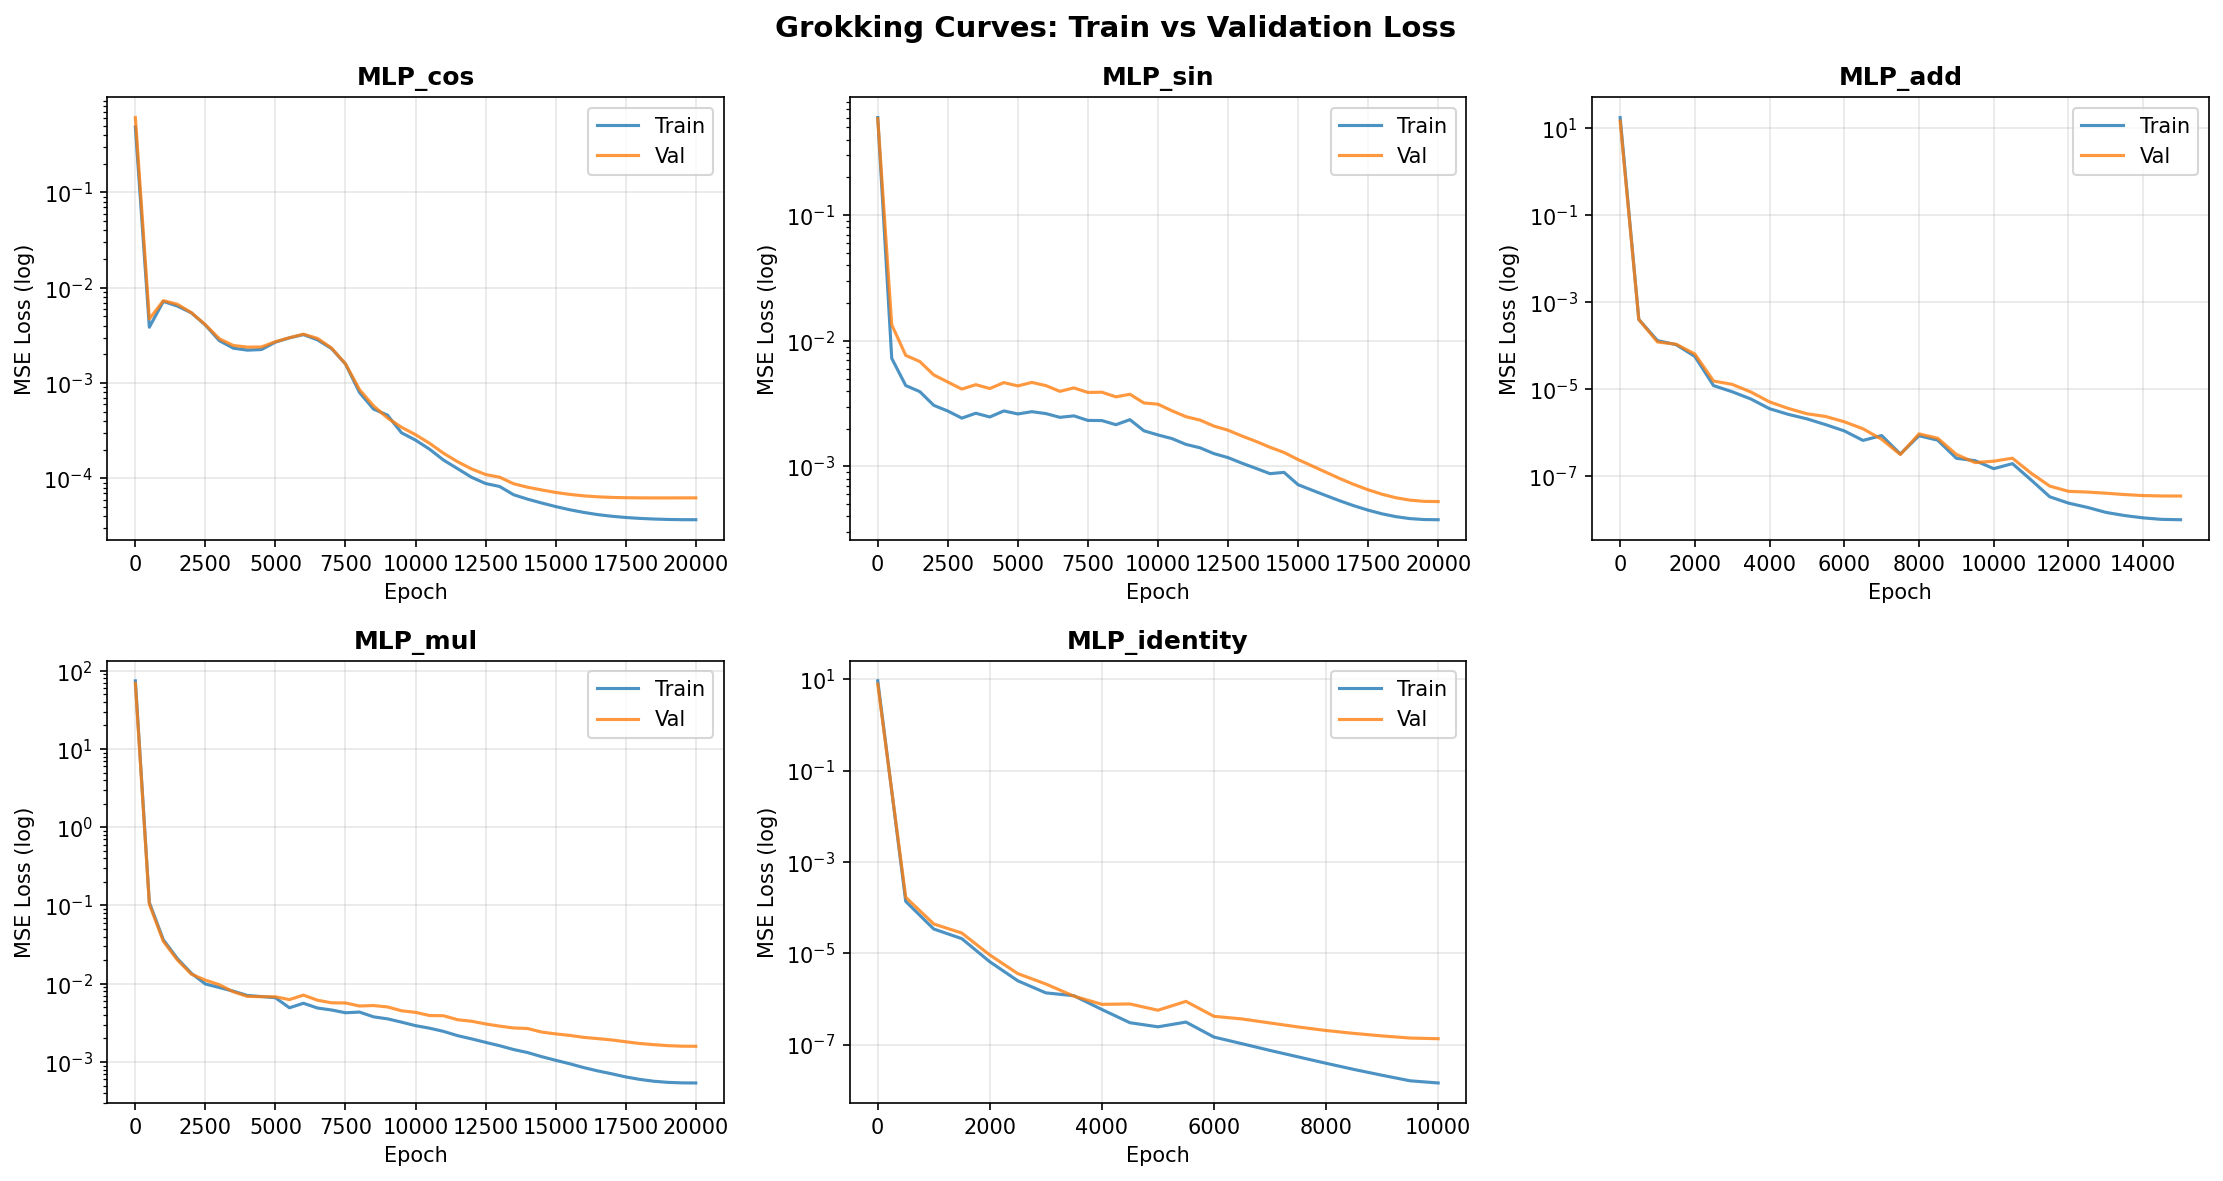
\includegraphics[width=0.7\linewidth]{grokking_curves.png}
    \caption{Training vs.\ validation loss illustrating grokking.}
\end{figure}
\end{frame}

\makepart{Method}

\section{Pipeline}

\begin{frame}{Pipeline Overview}
\begin{enumerate}
    \item \textbf{Phase 1.} Grok the MLPs (one per math operation).
    \item \textbf{Phase 2.} Build $\boldsymbol{\Theta}$ by evaluating MLPs on data.
    \item \textbf{Phase 3.} Discover sparse coefficients.
        \begin{itemize}
            \item \emphasize{Path A:} STLSQ (classical).
            \item \emphasize{Path B:} Gumbel-Softmax routing (differentiable).
        \end{itemize}
    \item \textbf{Phase 4.} Symbolic distillation via PySR.
\end{enumerate}
\end{frame}

\subsection{Least Squares}

\begin{frame}{Primer: Least Squares}
For data $(x_t, v_t, a_t)$, find $\xi$ minimizing total squared error:
\begin{equation*}
    \min_{\xi}\; \sum_t \bigl(a_t - [\xi_1 + \xi_2 x_t + \xi_3 v_t + \xi_4 x_t^2]\bigr)^2
\end{equation*}
Closed form:
\begin{equation*}
    \xi = (\boldsymbol{\Theta}^\top \boldsymbol{\Theta})^{-1} \boldsymbol{\Theta}^\top a.
\end{equation*}
\end{frame}

\subsection{Sparse Regression}

\begin{frame}{Primer: Sparse Regression}
Plain least squares fits \alert{all} coefficients (most slightly nonzero from noise).\\[0.3cm]
\emphasize{Sparse regression} prefers solutions where most coefficients are exactly zero -- because real laws are short.\\[0.3cm]
\textbf{STLSQ} (Sequentially Thresholded Least Squares):
\begin{enumerate}
    \item Run least squares.
    \item Zero out any $|\xi_i| < $ threshold.
    \item Refit on survivors.
    \item Repeat.
\end{enumerate}
\end{frame}

\begin{frame}{STLSQ on the Spring (Toy)}
Truth: $\dot{v} = -2x - 0.3v$. Library: $[1, x, v, x^2]$. Threshold $=0.1$.
\begin{table}
    \centering
    \begin{tabular}{@{}ll@{}}
        \toprule
        Step & Coefficients \\
        \midrule
        Iter 1 (LSQ)   & $[\,0.05,\;-1.95,\;-0.28,\;0.03\,]$ \\
        Threshold      & $[\,0,\;-1.95,\;-0.28,\;0\,]$ \\
        Iter 2 (refit) & $[\,0,\;-2.00,\;-0.30,\;0\,]$ \\
        \bottomrule
    \end{tabular}
\end{table}
Recovered: $\dot{v} = -2.00\,x - 0.30\,v$. \example{\textbf{Correct.}}
\end{frame}

\section{Phases 1 \& 2}

\begin{frame}{Phase 1: Grokking the Library}
Five small MLPs, one per operation:
\begin{equation*}
    \mathrm{identity}(x),\;\cos(x),\;\sin(x),\;\mathrm{add}(x,y),\;\mathrm{mul}(x,y)
\end{equation*}
Each trained on random samples until validation MSE $\sim 10^{-7}$.\\[0.3cm]
These \emphasize{frozen} MLPs become the columns of $\boldsymbol{\Theta}$.
\end{frame}

\begin{frame}{Phase 2: Neural Library Construction}
\textbf{Standard SINDy library:}
\begin{equation*}
    \boldsymbol{\Theta}(X) = [\,1,\;x,\;v,\;\sin(x),\;\dots\,]
\end{equation*}
\textbf{Neural SINDy library:}
\begin{align*}
    \boldsymbol{\Theta}(X) = [\, & \mathrm{id\_mlp}(x),\;\mathrm{id\_mlp}(v),\;\sin\mathrm{\_mlp}(x),\;\cos\mathrm{\_mlp}(x), \\
    & \mathrm{add\_mlp}(x,v),\;\mathrm{mul\_mlp}(x,v),\;\dots\,]
\end{align*}
Eight columns total in the paper's experiments.
\end{frame}

\makepart{Experiments and Results}

\section{Experimental Setup}

\begin{frame}{Experimental Setup}
\small
\textbf{System:} damped harmonic oscillator,\;
$\ddot{x} = -kx - c\dot{x}$,\; $k=1.0$,\; $c=0.1$.\\[0.1cm]
\textbf{Data:} 600 time points, $\Delta t = 0.05$, Gaussian noise $\sigma=0.001$.\\
\textbf{Initial conditions:} $x(0)=1.0,\; \dot{x}(0)=0.0$.
\begin{figure}
    \centering
    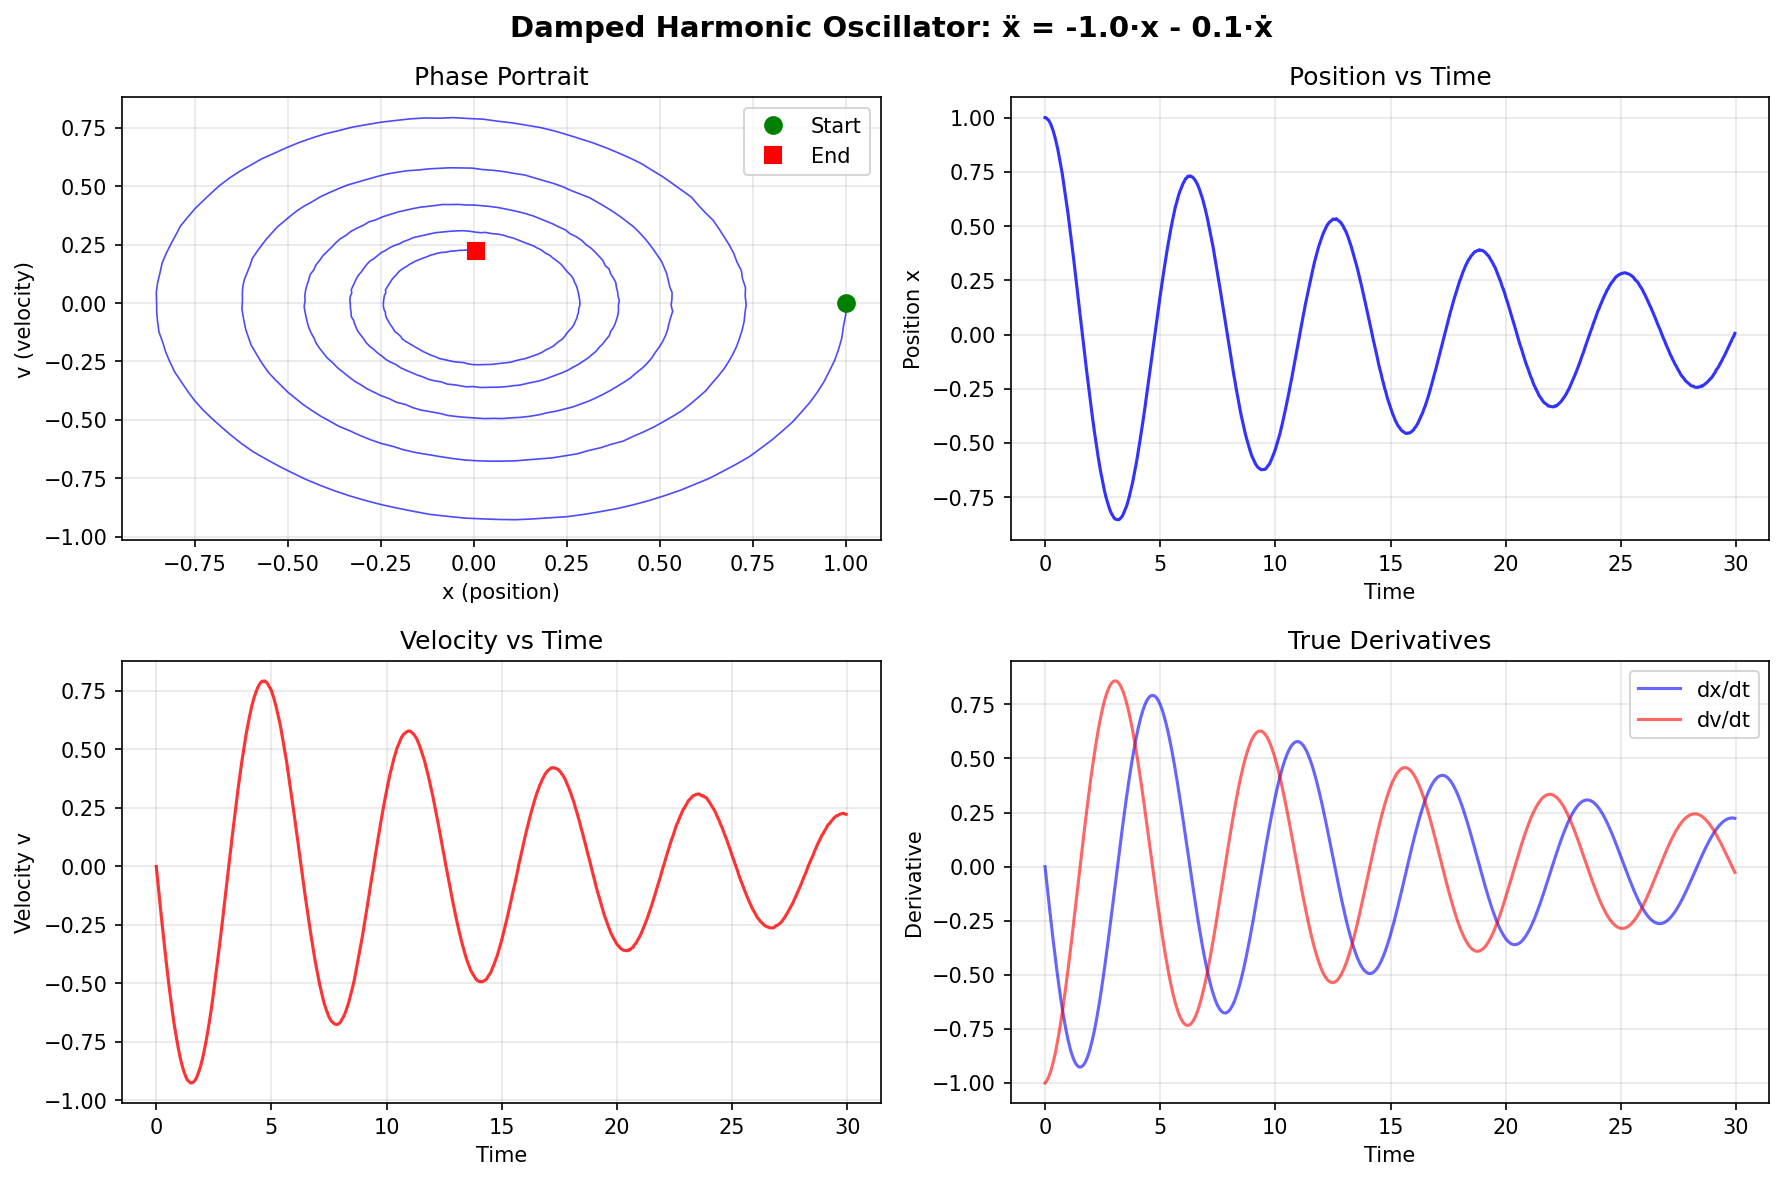
\includegraphics[width=0.65\linewidth]{oscillator_data.png}
\end{figure}
\end{frame}

\section{Path A: STLSQ}

\begin{frame}{Path A: STLSQ Result}
\small
After STLSQ on the 8-term neural library:
\begin{align*}
    \dot{x} &= -0.33\,\mathrm{id}(x) + 0.67\,\mathrm{id}(v) + 0.33\,\mathrm{add}(x,v) \\
    \dot{v} &= -0.63\,\mathrm{id}(x) + 0.27\,\mathrm{id}(v) - 0.37\,\mathrm{add}(x,v)
\end{align*}
Substituting $\mathrm{add}(x,v)\approx x+v$:
\begin{align*}
    \dot{x} &\approx 0.9999\,v, \qquad \dot{v} \approx -0.9998\,x - 0.0999\,v.
\end{align*}
MSE $\approx 10^{-6}$, but \alert{6 of 16 coefficients nonzero}.
\begin{figure}
    \centering
    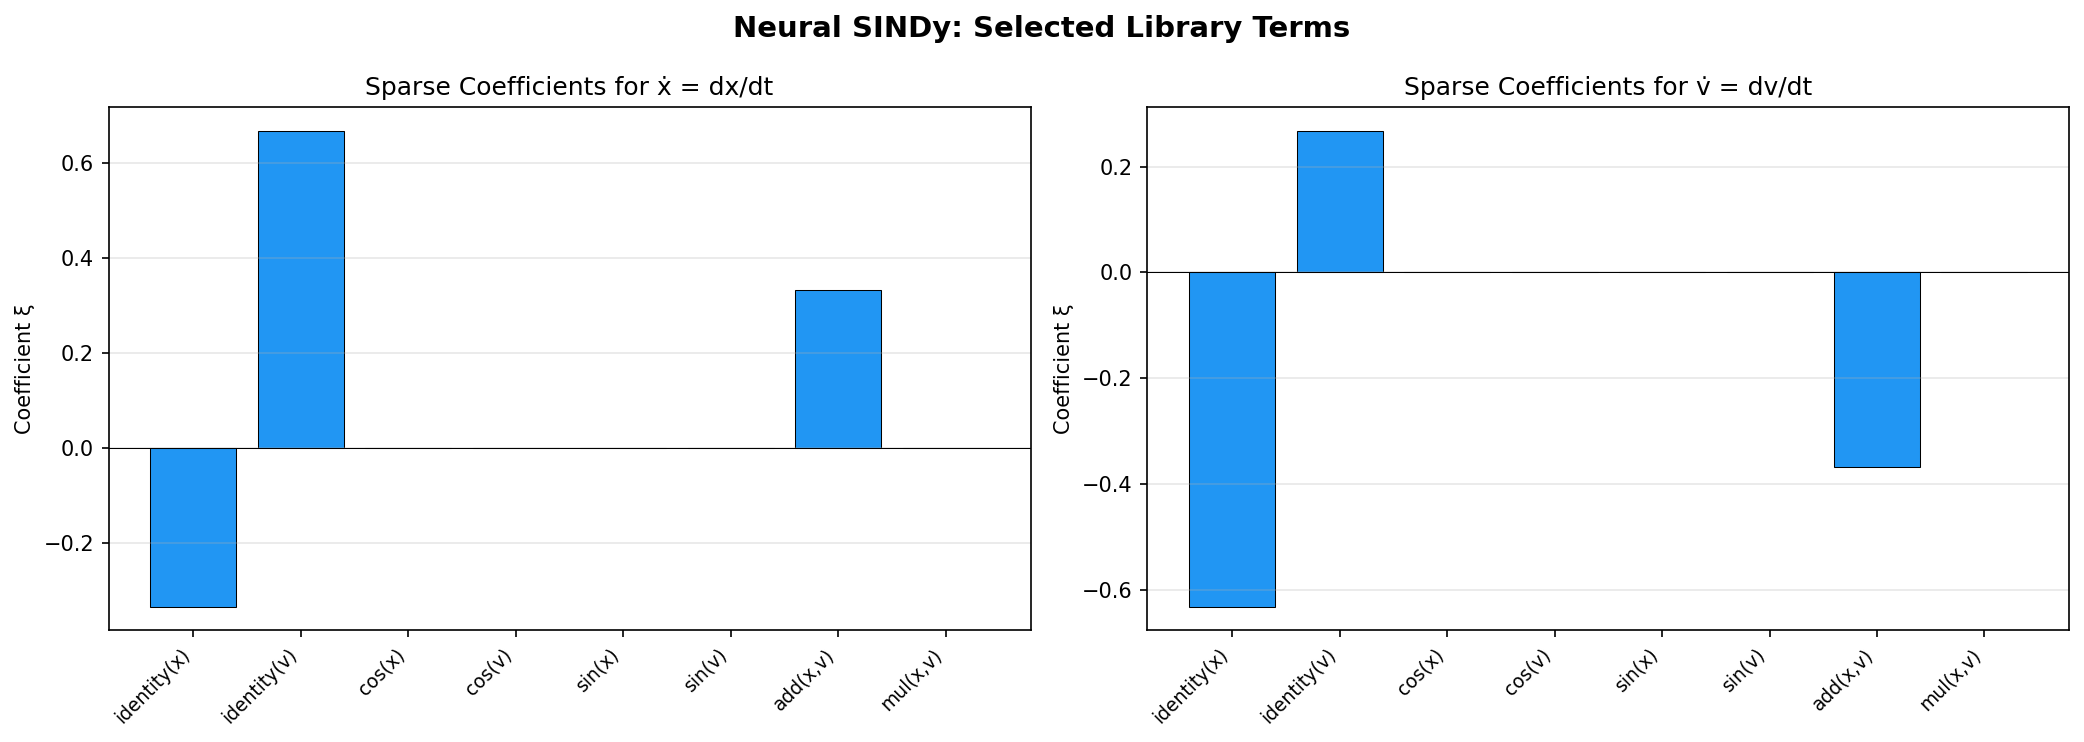
\includegraphics[width=0.55\linewidth]{coefficients.png}
\end{figure}
\end{frame}

\subsection{Collinearity}

\begin{frame}{Primer: Collinearity}
Two library columns are \alert{linearly dependent} when one equals a combination of others:
\begin{equation*}
    \mathrm{add}(x,v) \;\equiv\; \mathrm{id}(x) + \mathrm{id}(v).
\end{equation*}
$\boldsymbol{\Theta}$ becomes \emphasize{rank-deficient} $\Rightarrow$ infinitely many equally-good solutions $\Rightarrow$ STLSQ splits coefficients arbitrarily across redundant columns.\\[0.3cm]
Output is correct; \alert{individual coefficients lose interpretability}.
\end{frame}

\section{Path B: Gumbel-Softmax Routing}

\begin{frame}{Why Path B (Routing)?}
STLSQ has no notion of ``redundant terms.'' We need a selection mechanism that:
\begin{itemize}
    \item Picks a \emphasize{discrete} subset of basis functions.
    \item Stays \emphasize{differentiable} for gradient training.
    \item Can be biased toward \emphasize{simpler} terms.
\end{itemize}
\vspace{0.3cm}
Enter \example{Gumbel-Softmax routing}.
\end{frame}

\subsection{Gumbel-Softmax}

\begin{frame}{Primer: Gumbel-Softmax (1/2)}
A trick to make ``pick one discrete option'' differentiable.\\[0.3cm]
\textbf{Recipe:}
\begin{enumerate}
    \item Sample Gumbel noise $g_i \sim \mathrm{Gumbel}(0,1)$ per option.
    \item Add to logits: $\ell_i + g_i$.
    \item Divide by temperature $\tau$.
    \item Apply softmax.
\end{enumerate}
\begin{equation*}
    p_i = \frac{\exp((\ell_i + g_i)/\tau)}{\sum_j \exp((\ell_j + g_j)/\tau)}
\end{equation*}
\end{frame}

\begin{frame}{Primer: Gumbel-Softmax (2/2)}
Logits $\ell = [2.0,\;0.5,\;-1.0]$ for $[\mathrm{id},\sin,\cos]$.\\[0.3cm]
\textbf{High $\tau=5.0$ (early):} softmax $\approx [0.42,\,0.37,\,0.21]$ -- soft mixture, all gradients flow.\\[0.2cm]
\textbf{Low $\tau=0.05$ (late):} softmax $\approx [1.000,\,0.000,\,0.000]$ -- effectively one-hot.\\[0.3cm]
\textbf{Schedule:} $\tau$ anneals $5.0 \to 0.05$ over $2{,}500/4{,}000$ epochs.
\end{frame}

\begin{frame}{Primer: Straight-Through Estimator}
\textbf{Forward pass:} replace softmax with \emphasize{hard argmax} $\Rightarrow$ discrete behavior.\\[0.3cm]
\textbf{Backward pass:} pretend you used soft softmax $\Rightarrow$ \emphasize{gradients flow}.\\[0.3cm]
Without it, argmax has zero gradient and the router cannot learn.
\end{frame}

\begin{frame}{Why the Gumbel Noise Matters (Toy)}
Two terms tied at small displacement: $\sin(x)\approx x$ for $|x|<1$.\\[0.3cm]
\textbf{Without noise:} identical softmax every pass $\Rightarrow$ router locks onto whichever started slightly higher. No exploration.\\[0.3cm]
\textbf{With noise:} different sample-by-sample picks $\Rightarrow$ both terms get tested $\Rightarrow$ complexity prior breaks the tie.\\[0.3cm]
The noise is what makes Gumbel-Softmax actually \emphasize{sample} rather than smooth.
\end{frame}

\subsection{Router Variants}

\begin{frame}{Four Router Variants}
R1, R2, R3, R4 -- each fixing a flaw in the previous one.
\begin{table}
    \centering
    \small
    \begin{tabular}{@{}lllll@{}}
        \toprule
                & Routing           & $k$ & Prior                    & Result \\
        \midrule
        R1      & state-dependent   & 1   & none                     & misses damping       \\
        R2      & state-independent & 1   & none                     & $\sin/\mathrm{id}$ collapse \\
        R3      & state-independent & 2   & $\alpha=1.0$             & correct              \\
        R4      & state-independent & 2   & $\alpha=1.5$ + cond.\ ent. & correct              \\
        \bottomrule
    \end{tabular}
\end{table}
\end{frame}

\begin{frame}{R1: State-Dependent Router}
Logits depend on the state via a small MLP:
\begin{equation*}
    \ell(x,v) = \mathrm{MLP}_{\mathrm{router}}([x,v]).
\end{equation*}
\textbf{Problems:} $\sim 10{,}000$ params; routing varies per sample (\alert{violates SINDy global uniformity}); $k=1$ allows only one term per equation.\\[0.2cm]
\textbf{Recovers:} $\dot{x}=+1.0\,\mathrm{id}(v),\quad \dot{v} = -1.01\,\sin(x)$ -- damping missing.
\begin{figure}
    \centering
    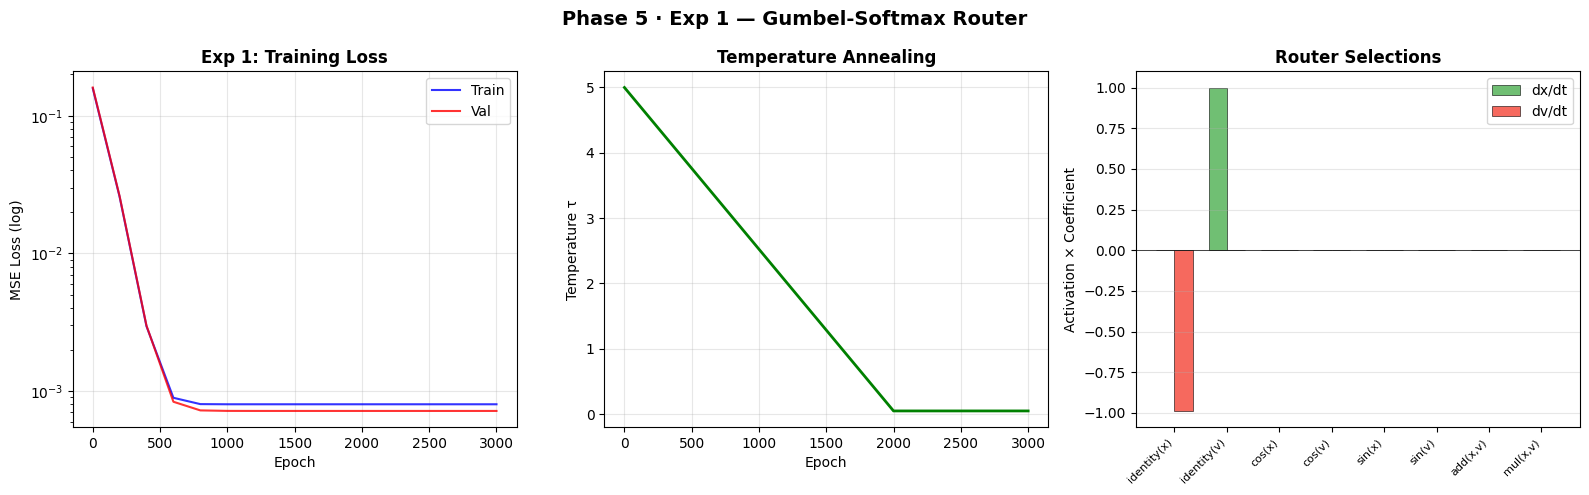
\includegraphics[width=0.6\linewidth]{phase_5_exp1_gumble_softmax_router.png}
\end{figure}
\end{frame}

\begin{frame}{R2: State-Independent Router}
One learnable logit vector per derivative, broadcast across all samples. \emphasize{Only 32 params.} Restores global uniformity.\\[0.2cm]
But: still $k=1$; no complexity prior $\Rightarrow$ \alert{collapses to $\sin(x)$ instead of $x$}.
\begin{align*}
    \dot{x} = +1.03\,\sin(v), \qquad \dot{v} = -1.01\,\sin(x).
\end{align*}
Symbolically misleading.
\begin{figure}
    \centering
    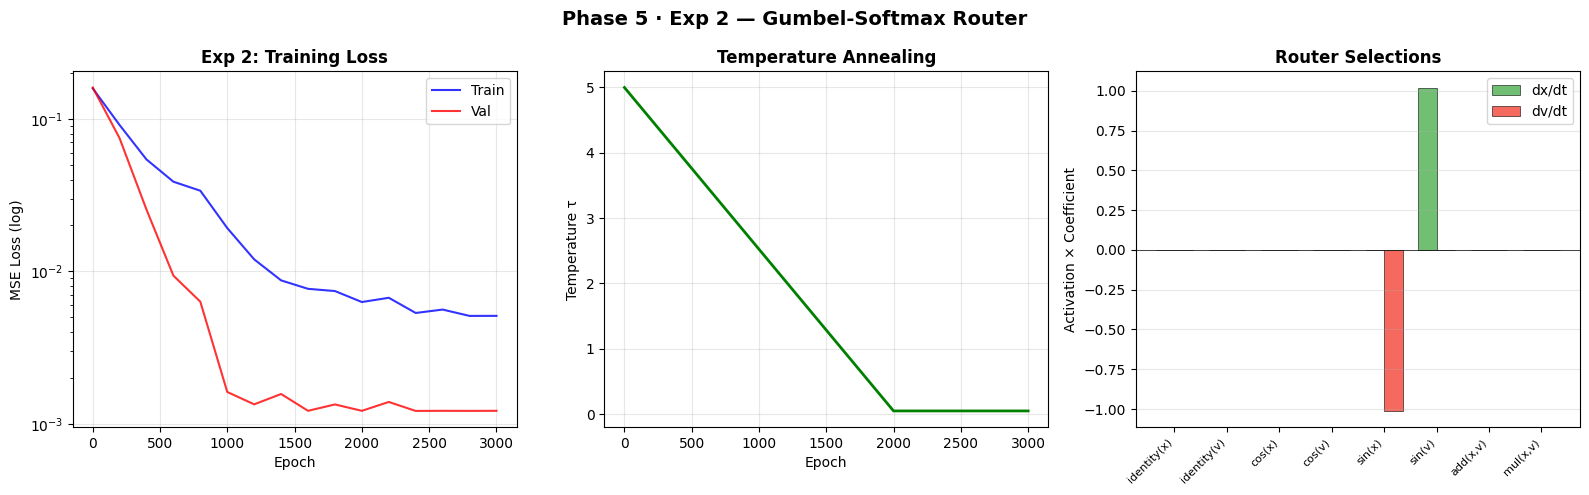
\includegraphics[width=0.55\linewidth]{phase_5_exp2_gumble_softmax_router.png}
\end{figure}
\end{frame}

\begin{frame}{The $\sin/\mathrm{identity}$ Collinearity (Toy)}
For $|x|<1$:
\begin{table}
    \centering
    \begin{tabular}{@{}rrr@{}}
        \toprule
        $x$    & $\sin(x)$ & error \\
        \midrule
        1.000 & 0.841 & 0.159 \\
        0.350 & 0.343 & 0.007 \\
        0.180 & 0.179 & 0.001 \\
        \bottomrule
    \end{tabular}
\end{table}
Columns are numerically interchangeable $\Rightarrow$ no data-driven way to prefer one. R2 picks whichever started higher.\\[0.2cm]
We need an \emphasize{explicit Occam's-razor bias}.
\end{frame}

\begin{frame}{R3 Fix (a): Top-$k$ Routing}
Pick $k=2$ terms per derivative via \emphasize{iterative masked sampling without replacement}:
\begin{enumerate}
    \item Sample slot 1 $\Rightarrow$ say $\sin(x)$.
    \item Mask it: $\ell_{\sin(x)} = -\infty$.
    \item Sample slot 2 from remaining $\Rightarrow$ say $\mathrm{id}(v)$.
\end{enumerate}
\vspace{0.3cm}
Now $\dot{v}$ can have \emphasize{two terms}, enabling damping.
\end{frame}

\begin{frame}{R3 Fix (b): Complexity Prior}
Add a fixed bias to logits based on simplicity:
\begin{table}
    \centering
    \begin{tabular}{@{}lc@{}}
        \toprule
        Term       & Bias        \\
        \midrule
        identity   & $+\alpha$   \\
        $\sin,\cos$ & $0$         \\
        add, mul   & $-\alpha$   \\
        \bottomrule
    \end{tabular}
\end{table}
\textbf{Toy:} raw logits $[1.0,1.1,0.5,0.2]$ for $[\mathrm{id}(x),\sin(x),\mathrm{id}(v),\mathrm{add}]$ become $[2.0,1.1,1.5,-0.8]$ with $\alpha=1.0$. \example{Identity wins the tie.}\\[0.2cm]
\alert{Note:} the prior is \emphasize{manual}. Future work: automate via node count or MDL.
\end{frame}

\begin{frame}{R3 Result}
\begin{align*}
    \dot{x} &= +0.9999\,\mathrm{id}(v) \\
    \dot{v} &= -0.9997\,\mathrm{id}(x) - 0.0998\,\mathrm{id}(v)
\end{align*}
Correct to four decimal places. Only 48 params.\\[0.2cm]
But: stochastic Gumbel sampling at val time produced \alert{spikes up to $1000\times$} the surrounding floor.
\begin{figure}
    \centering
    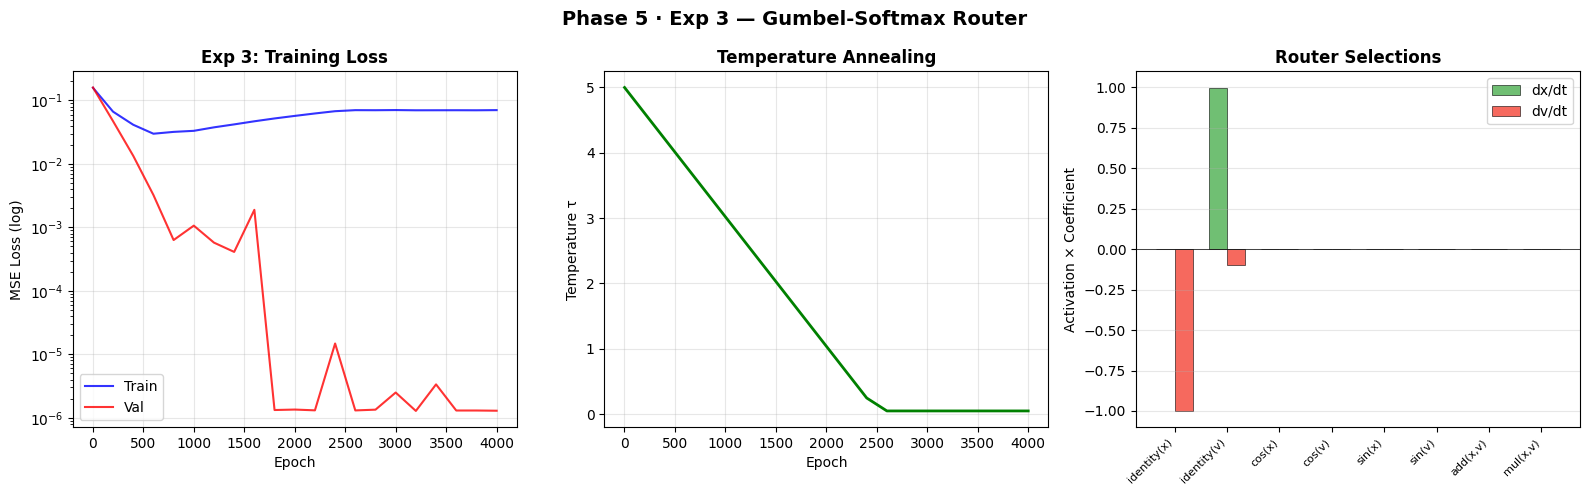
\includegraphics[width=0.6\linewidth]{phase_5_exp3_gumble_softmax_router.png}
\end{figure}
\end{frame}

\subsection{R4 and Validation}

\begin{frame}{Primer: Conditional Slot Entropy (R4)}
\textbf{Original (R3) entropy regularizer:} penalized the entropy of the \alert{base} logits -- before masking. After slot 1 committed, slot 2's conditional distribution stayed flat.\\[0.3cm]
\textbf{R4 fix:} penalize \emphasize{each slot's conditional distribution as the mask advances} -- mirroring the forward pass.\\[0.3cm]
This forces \emphasize{every} slot to commit independently. Damping coefficient now lands cleanly.\\[0.2cm]
\example{\textbf{Substantive contribution of the routing pipeline.}}
\end{frame}

\begin{frame}{Primer: Deterministic Validation}
Standard Gumbel-Softmax draws fresh noise every forward pass -- including at validation. Single unlucky draws caused $100\times$--$1000\times$ val-MSE spikes.\\[0.3cm]
\textbf{Fix:} add a hard-argmax evaluation path, used \emphasize{only at val time}.
\begin{itemize}
    \item Training: stays stochastic (optimization unchanged).
    \item Validation: deterministic, reproducible.
\end{itemize}
\begin{figure}
    \centering
    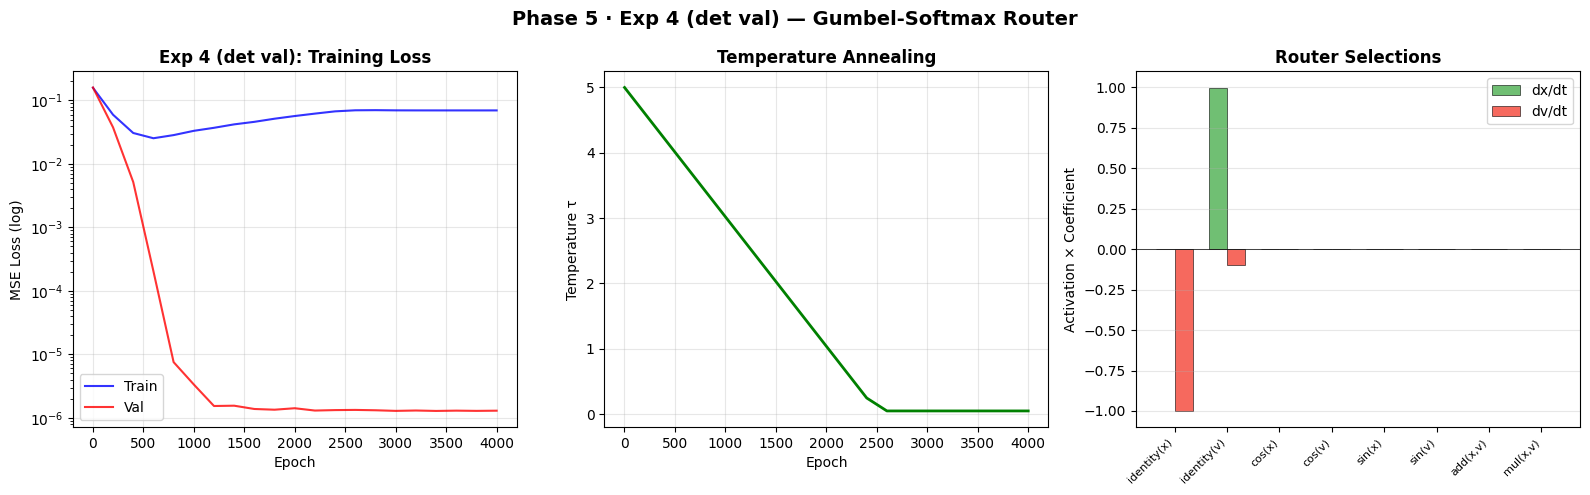
\includegraphics[width=0.45\linewidth]{phase_5_exp3(det_val)_gumble_softmax_router.png}
    \hfill
    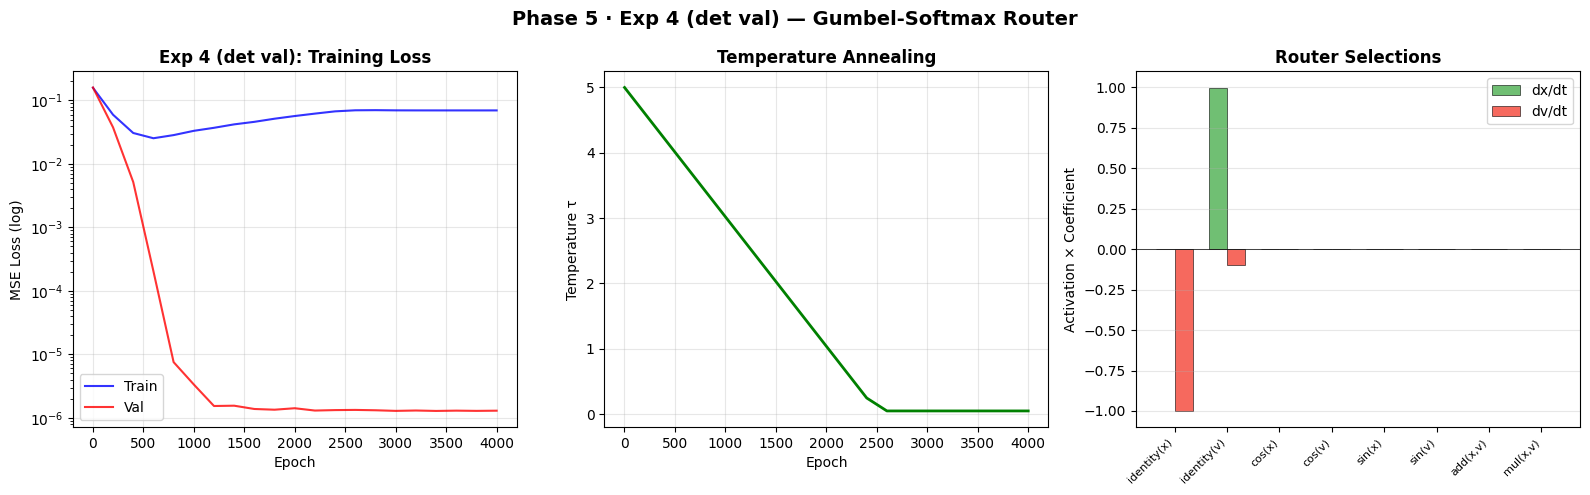
\includegraphics[width=0.45\linewidth]{phase_5_exp4(det_val)_gumble_softmax_router.png}
\end{figure}
\end{frame}

\begin{frame}{Why Training Goes Up While Validation Goes Down}
\textbf{Training loss} $=$ reconstruction MSE $+$ entropy $+$ complexity penalties.\\
\textbf{Validation loss} $=$ reconstruction MSE only (deterministic argmax).\\[0.2cm]
The penalty weight $\eta(\tau) = \eta_{\max}(1 - \tau/\tau_{\mathrm{start}})$ \emphasize{grows} as $\tau$ anneals.
\begin{table}
    \centering
    \small
    \begin{tabular}{@{}rrrrrr@{}}
        \toprule
        Epoch & Recon & $\eta$ & Penalties & Train & Val \\
        \midrule
        600   & 0.02      & 0.05 & 0.0015 & 0.0215 & 0.02 \\
        2000  & $10^{-4}$ & 0.4  & 0.035  & 0.035  & $10^{-4}$ \\
        4000  & $10^{-6}$ & 1.0  & 0.055  & 0.055  & $10^{-6}$ \\
        \bottomrule
    \end{tabular}
\end{table}
\alert{Not a generalization gap} -- two different objectives plotted on the same axes.
\end{frame}

\section{Final Results}

\begin{frame}{Final Results Table}
\centering
\scriptsize
\begin{tabular}{@{}lrcll@{}}
    \toprule
    Variant                                              & Params      & Val MSE                & $\dot{x}$           & $\dot{v}$ \\
    \midrule
    R1 (state-dep, $k=1$)                                & $9{,}760$   & $9.8 {\times} 10^{-4}$ & $+1.0000\,v$        & $-1.0138\,\sin(x)$ \\
    R2 (state-indep, $k=1$)                              & $32$        & $1.2 {\times} 10^{-3}$ & $+1.0265\,\sin(v)$  & $-1.0138\,\sin(x)$ \\
    R3 (top-2, $\alpha{=}1.0$, det.\ val)                & $48$        & $1.0 {\times} 10^{-6}$ & $+0.9999\,v$        & $-0.9998\,x - 0.0996\,v$ \\
    R4 (top-2, $\alpha{=}1.5$, cond.\ ent., det.\ val)   & $48$        & $1.0 {\times} 10^{-6}$ & $+0.9998\,v$        & $-0.9998\,x - 0.0997\,v$ \\
    \midrule
    Truth                                                & ---         & ---                    & $+1.0\,v$           & $-1.0\,x - 0.1\,v$ \\
    \bottomrule
\end{tabular}
\vspace{0.5cm}
\begin{figure}
    \centering
    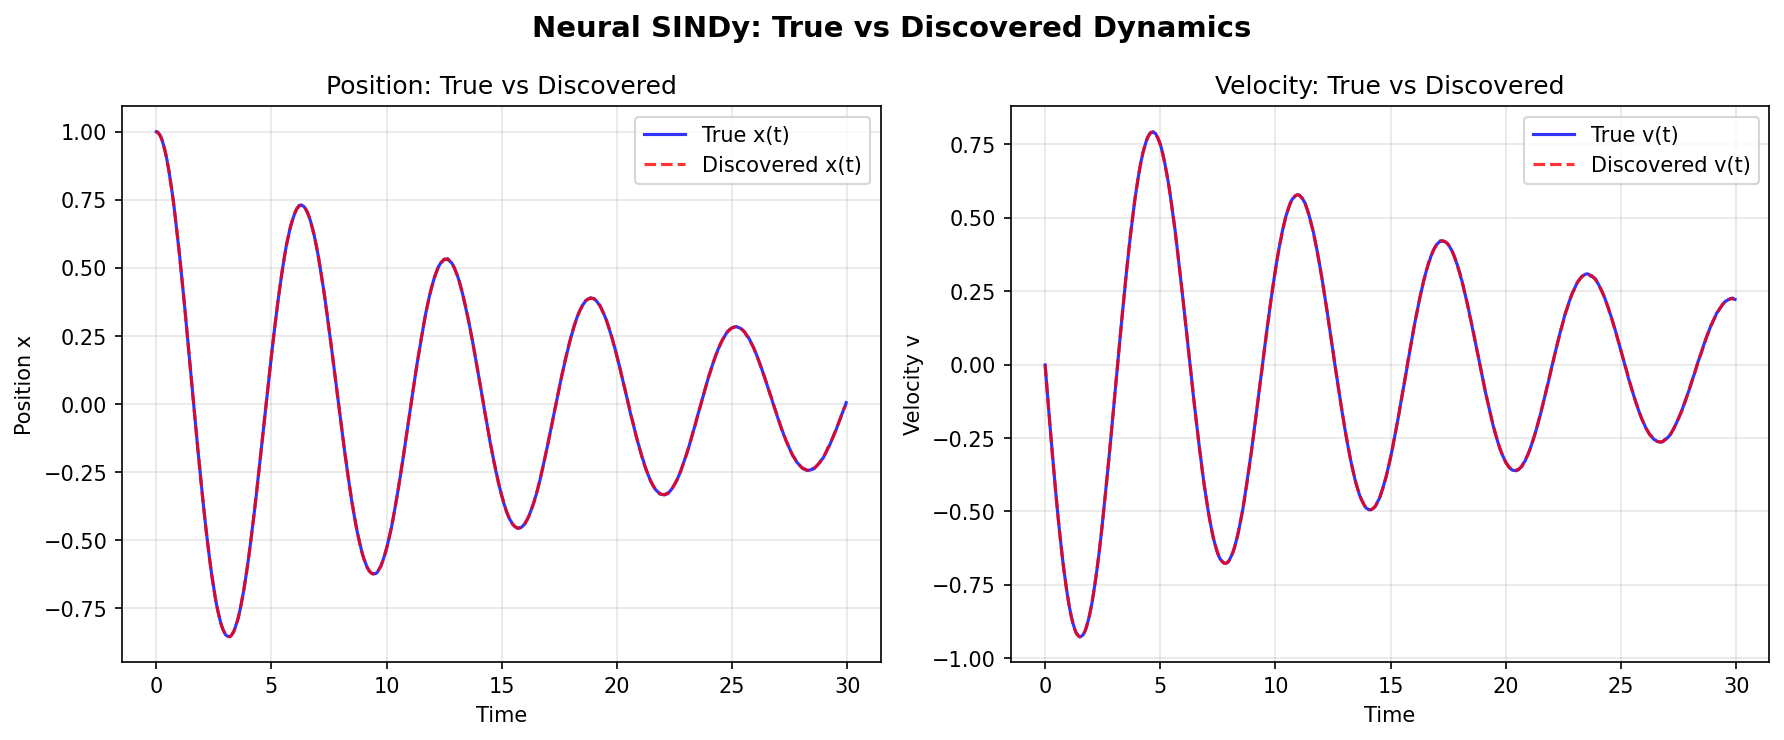
\includegraphics[width=0.55\linewidth]{discovery_comparison.png}
\end{figure}
\end{frame}

\section{Phase 4 and Ablations}

\begin{frame}{Phase 4: Symbolic Distillation}
After routing picks a winning MLP, distill it back to symbols using \emphasize{PySR} (genetic programming over expression trees).\\[0.3cm]
\textbf{Toy:} probe $\sin\mathrm{\_mlp}$ on a grid $\to$ table of $(x,y)$ pairs $\to$ PySR searches:
\begin{itemize}
    \item $x$ -- bad fit
    \item $x - x^3/6$ -- close
    \item $\sin(x)$ -- near-perfect, very short \example{\checkmark}
\end{itemize}
\vspace{0.3cm}
\textbf{Status:} described in methodology, \alert{not yet integrated end-to-end}. Listed as future work.
\end{frame}

\begin{frame}{Ablation: $\alpha=1.0$ vs.\ $\alpha=1.5$}
Once \emphasize{conditional slot entropy} is in place, the two settings produce statistically indistinguishable equations:
\begin{itemize}
    \item R3 ($\alpha=1.0$): $\dot{v} = -0.9998\,x - 0.0996\,v$
    \item R4 ($\alpha=1.5$): $\dot{v} = -0.9998\,x - 0.0997\,v$
\end{itemize}
\vspace{0.3cm}
\example{Conditional slot entropy is the substantive contribution} -- the prior strength is cosmetic at this precision.
\end{frame}

\makepart{Wrap-up}

\section{Takeaways}

\begin{frame}{Takeaways}
\begin{enumerate}
    \item Grokked MLPs \emphasize{can serve as a SINDy library} and recover true dynamics to $\sim 10^{-6}$ MSE.
    \item Naive neural libraries surface \emphasize{two flavors of collinearity} ($\mathrm{add} \equiv \mathrm{id}+\mathrm{id}$; $\sin \approx \mathrm{id}$ at small input) that STLSQ cannot resolve.
    \item \emphasize{Differentiable routing} with Gumbel-Softmax handles selection -- but only with top-$k$, complexity prior, and conditional slot entropy.
    \item \emphasize{Conditional slot entropy} is the substantive methodological contribution.
    \item Training-vs-validation inversion is \emphasize{expected} -- different objectives, not a generalization gap.
\end{enumerate}
\end{frame}

\section{Limitations and Future Work}

\begin{frame}{Limitations and Future Work}
\begin{itemize}
    \item \alert{Tested on one system.} Damped oscillator only -- needs higher-dim systems.
    \item \alert{Complexity prior is manual.} Should automate via node count / MDL.
    \item \alert{PySR not yet integrated.} Phase 4 is methodology, not yet code.
    \item \alert{Noise robustness.} Only $\sigma=0.001$ tested -- needs a sweep.
    \item \alert{Grokked basis quality.} All MLPs trained to MSE $\sim 10^{-7}$; weaker grokking would propagate noise into routing.
\end{itemize}
\end{frame}

\section{Future Work: Differentiable Trees}

\begin{frame}{The Combinatorial-Explosion Wall}
Current pipeline routes over a \emphasize{flat} 8-term library.\\[0.2cm]
To discover nested equations like $\sin(x_1 + x_2)$, classical SINDy must pre-compute every depth-$D$ composition.
\begin{itemize}
    \item Library size scales as $\mathcal{O}(N^D)$ with $N$ operators and depth $D$.
    \item Even modest $N{=}10$, $D{=}4$ blows past $10^4$ columns.
\end{itemize}
\vspace{0.2cm}
\alert{This is the wall a flat library hits, including ours.}
\end{frame}

\begin{frame}{Stacked Gumbel-Softmax Routing Trees}
Replace the flat library with a \emphasize{multi-layer routing tree} of grokked MLPs.
\begin{itemize}
    \item Each layer holds only base operators (e.g., $+,\,\times,\,\sin,\,\cos$).
    \item A Gumbel-Softmax router \cite{b7} between layers acts as a differentiable switchboard.
    \item Soft probabilistic routing at high $\tau$, snapping to discrete paths as $\tau \to 0$.
\end{itemize}
\vspace{0.2cm}
\textbf{Memory:} $\mathcal{O}(N \cdot D)$ instead of $\mathcal{O}(N^D)$ -- linear, not combinatorial.\\[0.2cm]
Conceptually adjacent to EQL \cite{b8}, VaSST \cite{b9}, and Symbolic-KAN \cite{b10}; \example{novelty here is grokked MLPs as the per-layer primitives}.
\end{frame}

\begin{frame}{Toy Example: Discovering $y = \sin(x_1 + x_2)$}
\textbf{Layer 0 (inputs):} $x_1,\, x_2$.\\[0.2cm]
\textbf{Layer 1 (binary ops):} $\mathrm{add\_mlp},\, \mathrm{mul\_mlp}$.
\begin{itemize}
    \item Router $\mathbf{W}^{(1)}$ chooses inputs for each binary op.
    \item Snaps to: $h_1 = \mathrm{add\_mlp}(x_1, x_2) \approx x_1 + x_2$.
\end{itemize}
\textbf{Layer 2 (unary ops):} $\sin\mathrm{\_mlp},\, \cos\mathrm{\_mlp}$.
\begin{itemize}
    \item Router $\mathbf{W}^{(2)}$ picks among Layer-0 and Layer-1 outputs.
    \item Snaps to: $y = \sin\mathrm{\_mlp}(h_1) \approx \sin(x_1 + x_2)$. \example{\checkmark}
\end{itemize}
\vspace{0.2cm}
Only $4$ primitives in memory, depth-$2$ nested expression recovered.
\end{frame}

\begin{frame}{Universal Gate Variant: Grokked EML}
A single binary operator suffices in principle:
\begin{equation*}
    \mathrm{eml}(x, y) = \exp(x) - \ln(y),
\end{equation*}
recently shown to generate \emphasize{every elementary function} via recursion.
\begin{itemize}
    \item \alert{Catch:} analytic EML is unstable -- $\ln(y)$ singularity at $0$, exponential drift.
    \item \emphasize{Our angle:} a \emphasize{grokked MLP} approximating EML smooths the singularity and bounds the gradients.
\end{itemize}
\vspace{0.2cm}
\textbf{Architectural simplification:} the routing tree becomes \emphasize{homogeneous} -- routers no longer pick operators, only operands.\\[0.2cm]
\textbf{Bonus:} EML structure admits a deterministic compiler back to algebraic notation -- \alert{may obviate PySR for Phase 4}.
\end{frame}

\begin{frame}{Proposed Roadmap}
\begin{enumerate}
    \item \emphasize{Ablation first.} Standard SINDy library + Gumbel routing vs.\ grokked-MLP library + Gumbel routing -- isolate the contribution of grokked primitives.
    \item \emphasize{Depth-2 tree} on a system with known nested structure (e.g., pendulum: $\ddot{\theta} = -(g/\ell)\sin\theta$).
    \item \emphasize{Grokked EML gate} as a single-primitive replacement for the heterogeneous library.
    \item \emphasize{Deterministic distillation} from EML routing paths as an alternative to PySR.
\end{enumerate}
\end{frame}

{
\setbeamertemplate{headline}{}
\setbeamertemplate{footline}{}
\begin{frame}[plain]
    \centering
    \vfill
    {\Huge Thank you.}\\[1cm]
    {\Large Questions?}
    \vfill
\end{frame}
}
\addtocounter{framenumber}{-1}

\begin{frame}[allowframebreaks]{References}
    \nocite{*}
    \printbibliography
\end{frame}

\end{document}
